\section{The actual product pairing and its two-support
radical}\label{the-actual-product-pairing-and-its-two-support-radical}

\begin{figure}
\centering
\pandocbounded{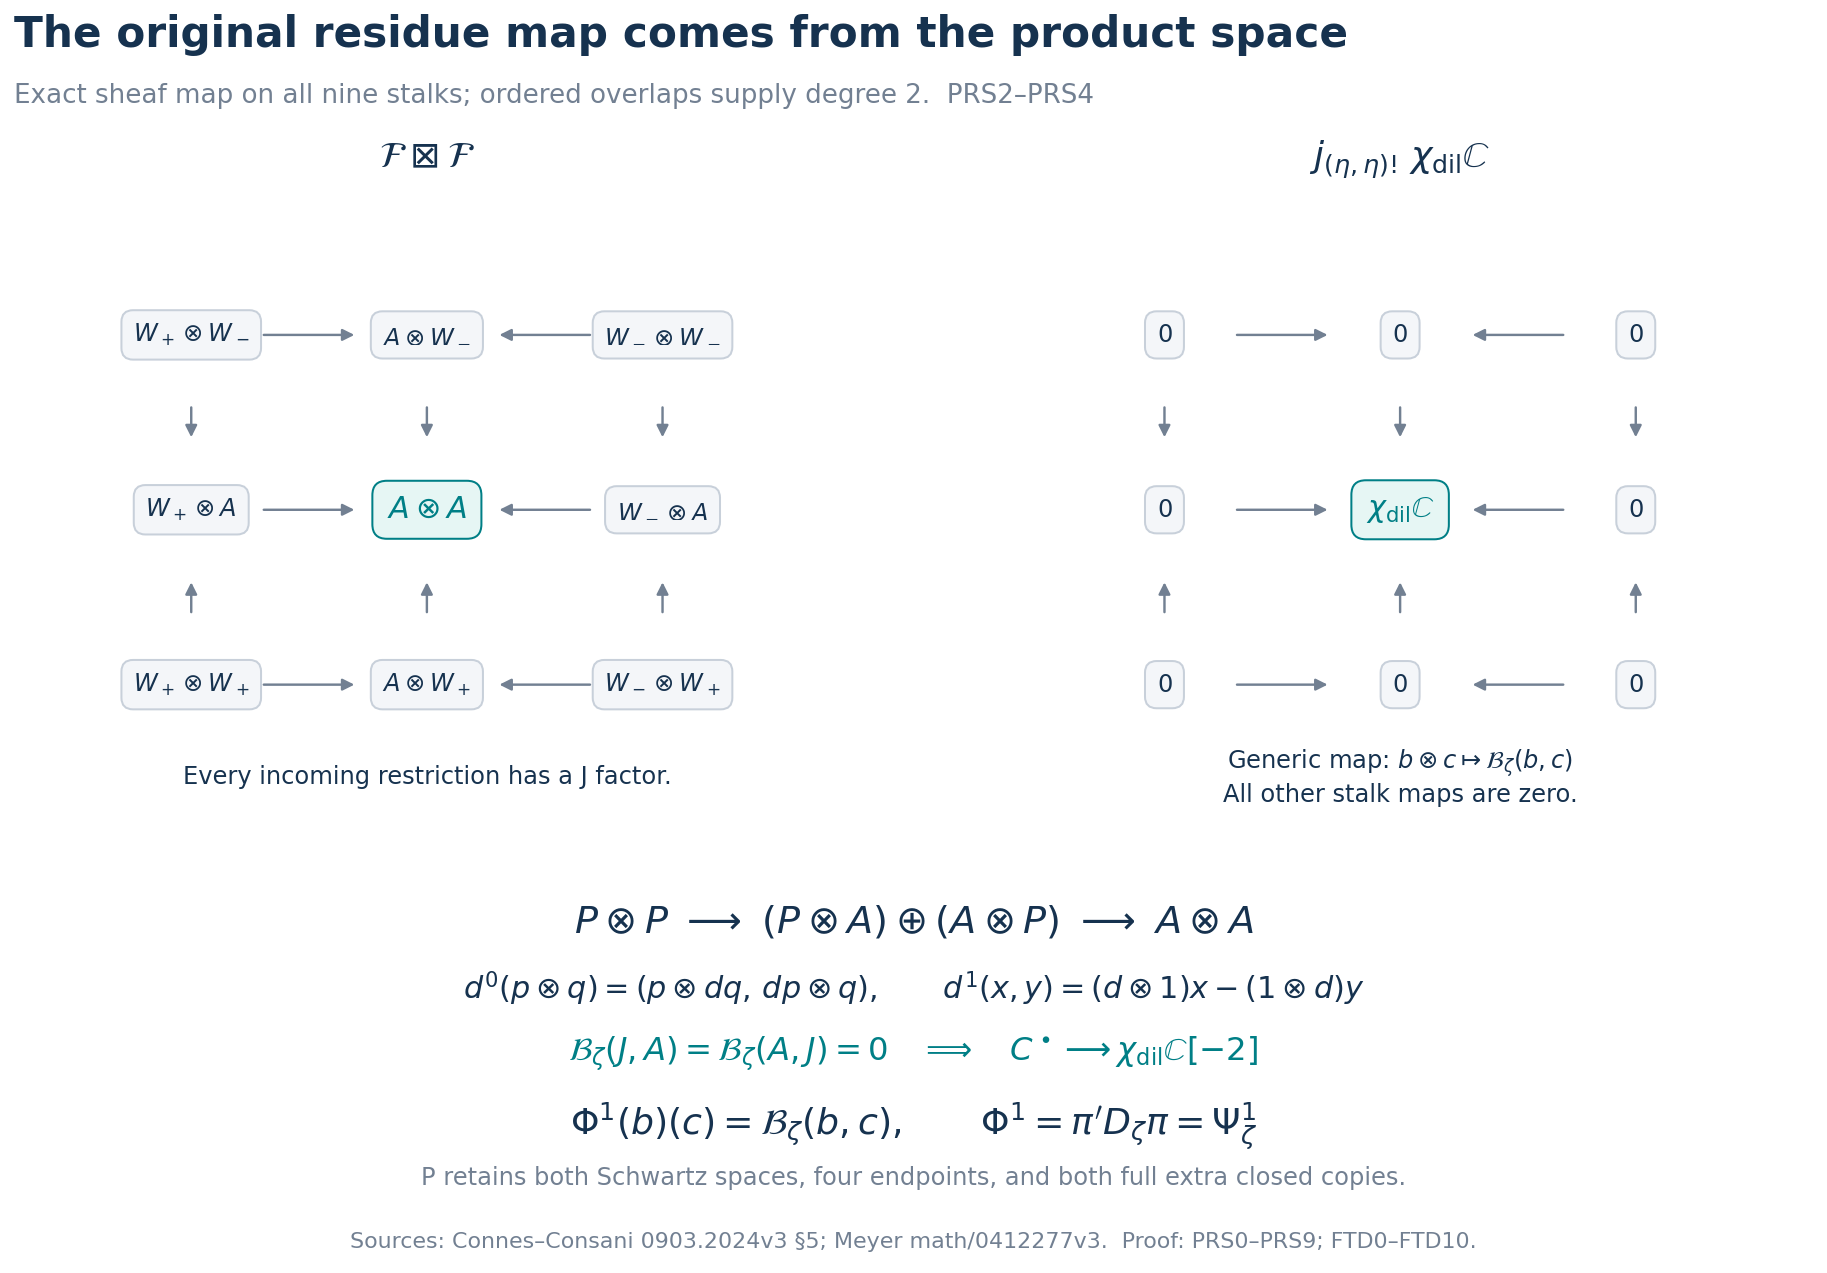
\includegraphics[keepaspectratio,alt={All nine stalks of the product pairing}]{ORIGINAL_RESIDUE_PRODUCT_SPACE.png}}
\caption{All nine stalks of the product pairing}
\end{figure}

Figure 1. The two diagrams are the actual external tensor and
extension-by-zero target on the original three-point product. Every
arrow into the generic pair contains an original restriction whose image
is J. The original residue form kills it in either slot. The ordered
product Čech complex, all signs, trace and exact return to the global
map are proved in
\href{https://github.com/KokunoYumeto/zeta-function-research-reader/blob/main/workbenches/splitzero-tandem/continuations/20260925-full-source-tensor-and-original-divisor/counterfactual/ORIGINAL_RESIDUE_PRODUCT_SHEAF_PAIRING.md}{PRS2--PRS4},
independently derived in
\href{https://github.com/KokunoYumeto/zeta-function-research-reader/blob/main/workbenches/splitzero-tandem/continuations/20260925-full-source-tensor-and-original-divisor/counterfactual/RESIDUE_PRODUCT_DIAGONAL_INDEPENDENT.md}{RPD2--RPD4}.
The independent proof keeps the Koszul identification with the external
projective resolution explicit. All endpoint and extra copies are
retained in P.

\begin{figure}
\centering
\pandocbounded{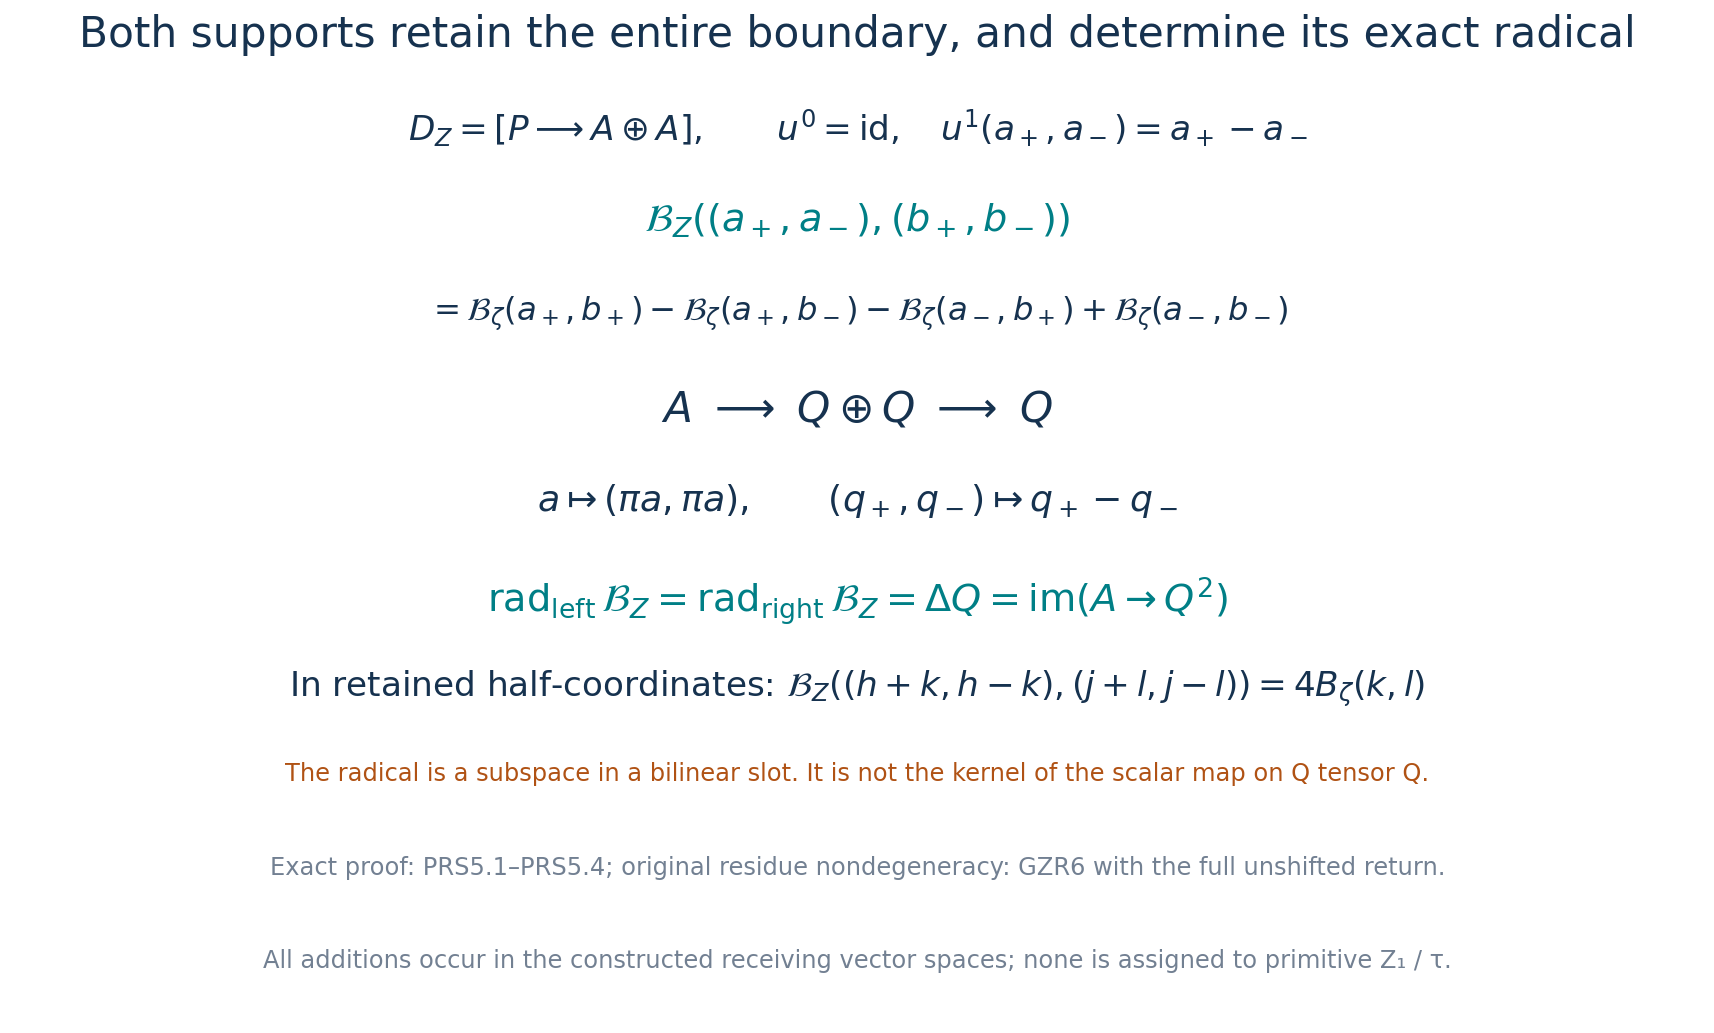
\includegraphics[keepaspectratio,alt={Both supports and the exact boundary radical}]{BOTH_SUPPORTS_RESIDUE_RADICAL.png}}
\caption{Both supports and the exact boundary radical}
\end{figure}

Figure 2.
\href{https://github.com/KokunoYumeto/zeta-function-research-reader/blob/main/workbenches/splitzero-tandem/continuations/20260925-full-source-tensor-and-original-divisor/counterfactual/ORIGINAL_RESIDUE_PRODUCT_SHEAF_PAIRING.md}{PRS5.1--PRS5.4}
proves the four-term supported form, its exact left and right radicals,
and the original diagonal/difference sequence. The coefficient four in
the retained half-coordinates is displayed. A bilinear radical is not
the entire kernel of the scalar map on a tensor product.
\href{https://github.com/KokunoYumeto/zeta-function-research-reader/blob/main/workbenches/splitzero-tandem/continuations/20260925-full-source-tensor-and-original-divisor/counterfactual/RESIDUE_PRODUCT_DIAGONAL_INDEPENDENT.md}{RPD7.4--RPD7.7}
constructs both distinct kernels for the diagonal calculation, including
an explicit scalar splitting using the full original zero germ.

\begin{figure}
\centering
\pandocbounded{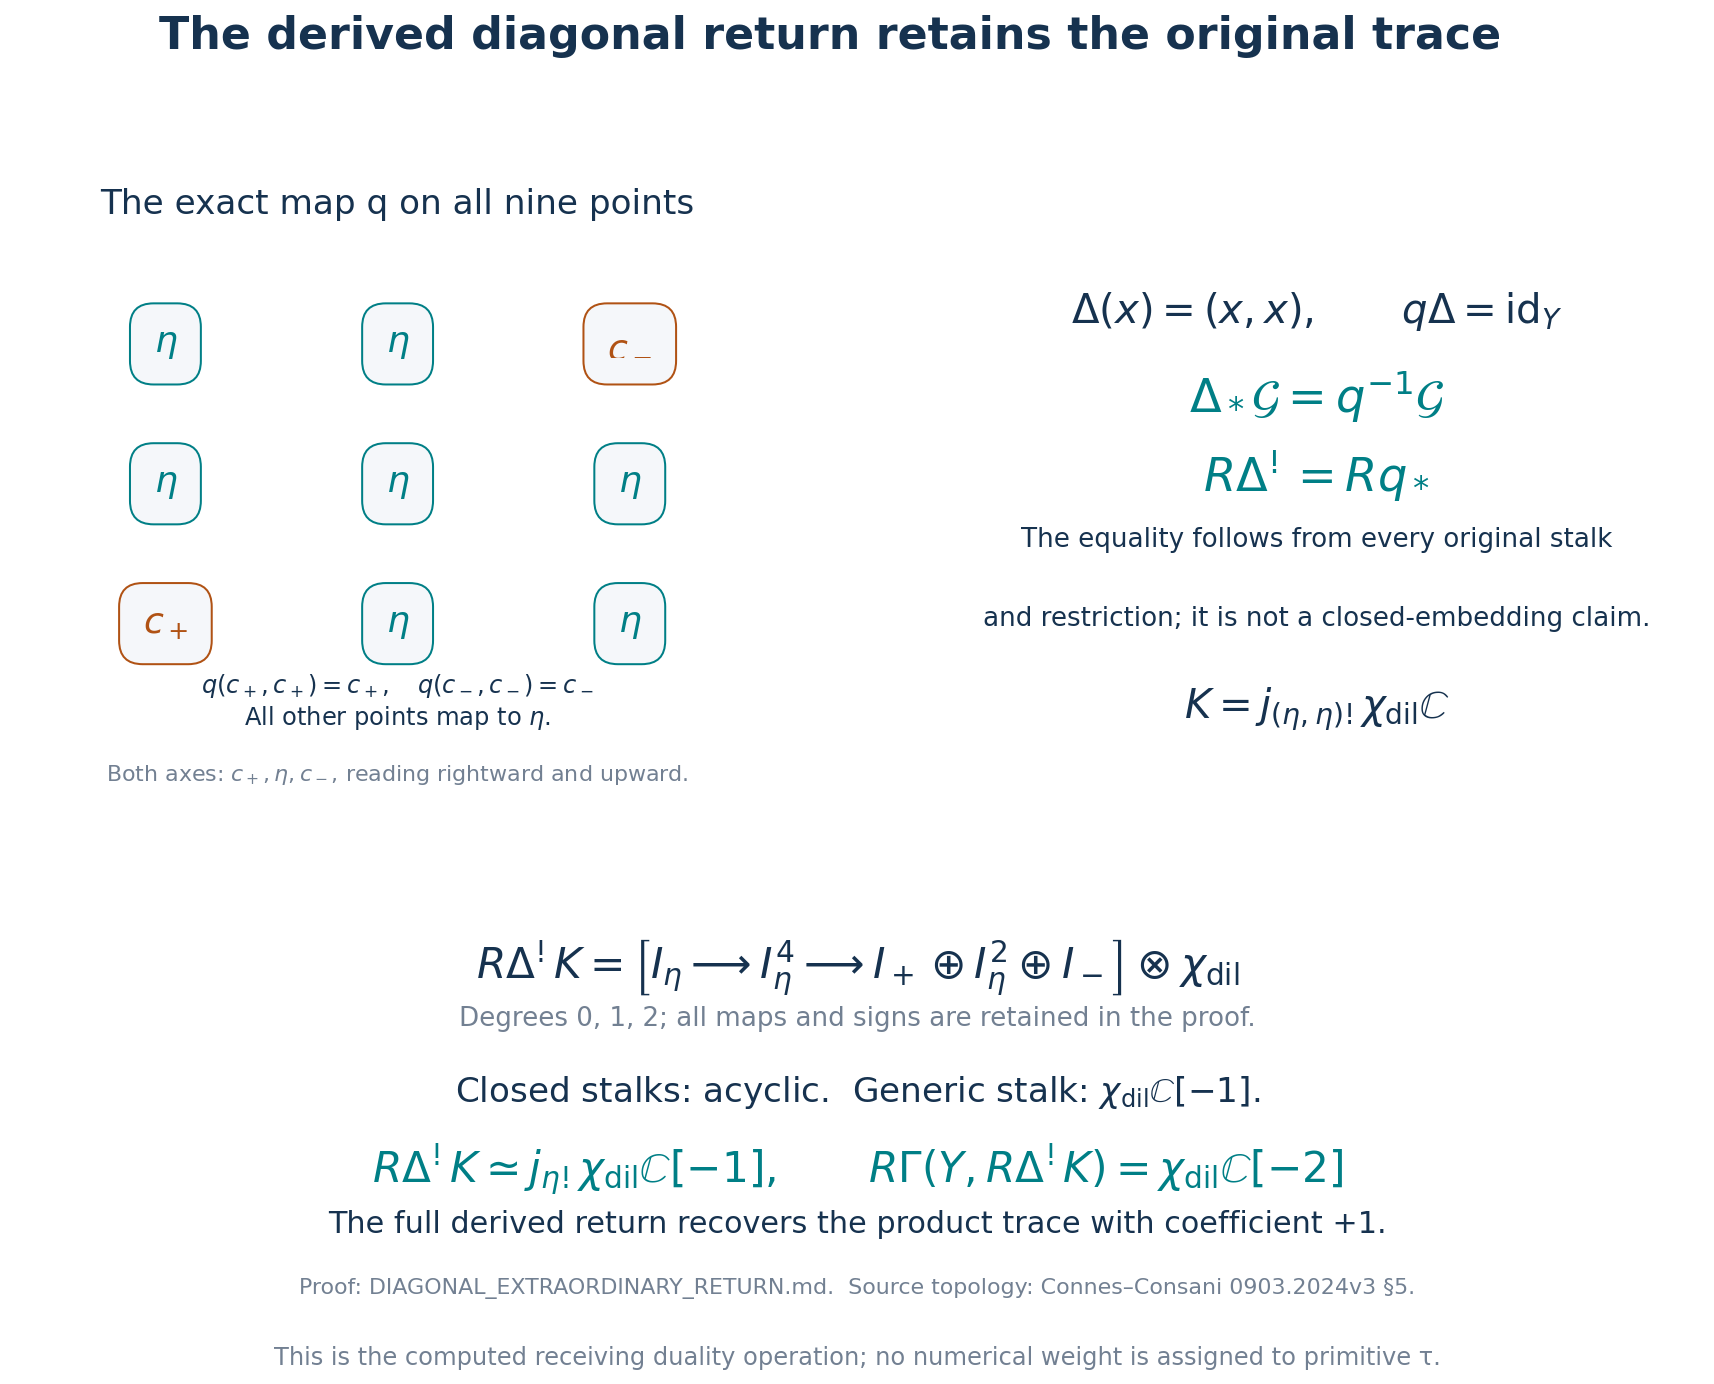
\includegraphics[keepaspectratio,alt={The actual derived diagonal return}]{DERIVED_DIAGONAL_TRACE_RETURN.png}}
\caption{The actual derived diagonal return}
\end{figure}

Figure 3. The map q is specified on all nine original points. The
identity Delta\_\emph{=q\^{}\{-1\} is proved on every sheaf stalk and
restriction. Its right adjoint is therefore Rq\_}, which gives the
complete displayed injective complex on the trace target. The exact
differentials, all three stalk complexes, a quasi-isomorphism and the
coefficient +1 trace return are proved in
\href{https://github.com/KokunoYumeto/zeta-function-research-reader/blob/main/workbenches/splitzero-tandem/continuations/20260925-full-source-tensor-and-original-divisor/counterfactual/DIAGONAL_EXTRAORDINARY_RETURN.md}{the
complete derived diagonal calculation}. The closed acyclic stalks remain
in that injective complex; the figure distinguishes its cohomology from
its complete representative. The source support and original dilation
character are retained.

\begin{figure}
\centering
\pandocbounded{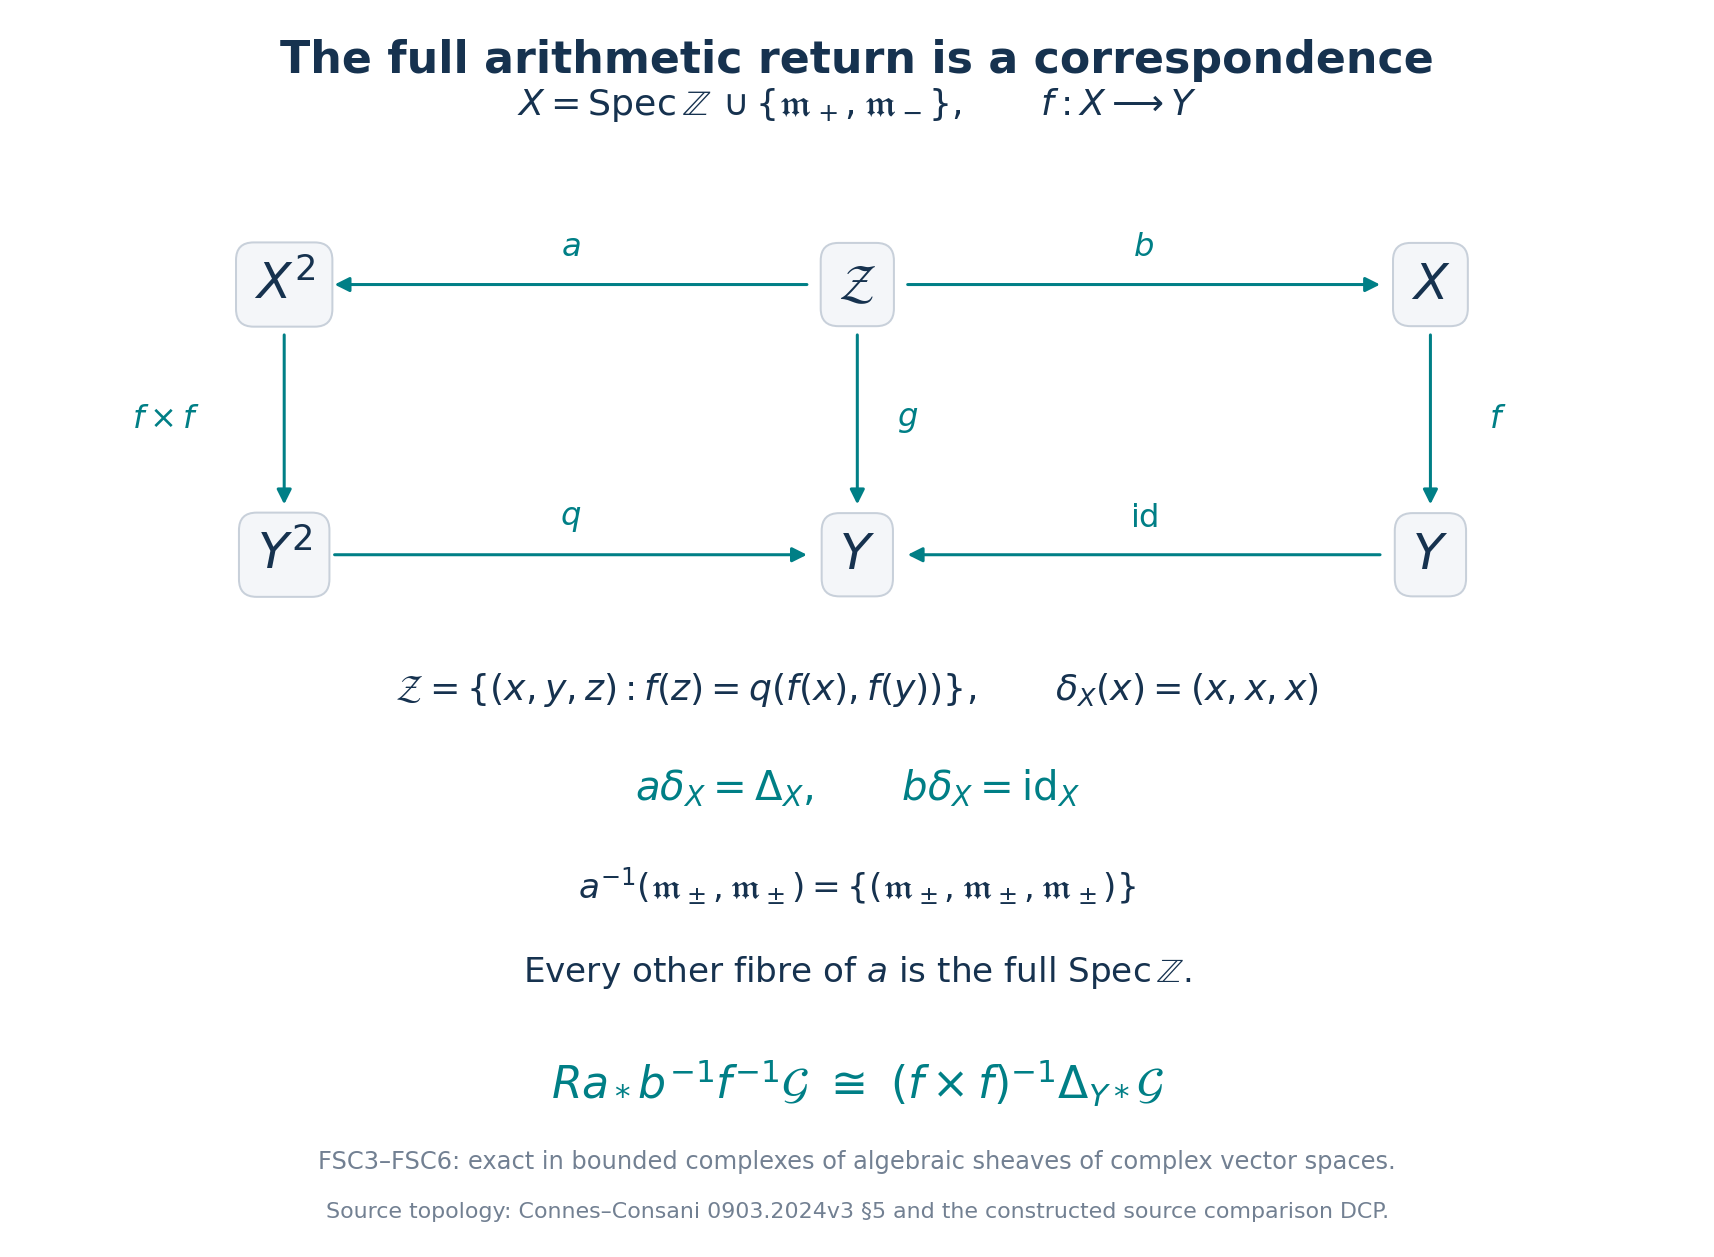
\includegraphics[keepaspectratio,alt={The full arithmetic source correspondence}]{FULL_SOURCE_DERIVED_CORRESPONDENCE.png}}
\caption{The full arithmetic source correspondence}
\end{figure}

Figure 4. The complete arithmetic source X, both projections of the
correspondence and every fibre are specified in
\href{https://github.com/KokunoYumeto/zeta-function-research-reader/blob/main/workbenches/splitzero-tandem/continuations/20260925-full-source-tensor-and-original-divisor/counterfactual/DERIVED_RETURN_FULL_SOURCE_CORRESPONDENCE.md}{FSC1--FSC6}.
The lifted diagonal retains each arithmetic point. FSC6 proves the
displayed derived coefficient isomorphism by an explicit injective
resolution, for bounded complexes of algebraic sheaves of complex vector
spaces. This is a proved comparison for those coefficients, not a
general proper-base-change assertion or a numerical weight theorem.

\begin{figure}
\centering
\pandocbounded{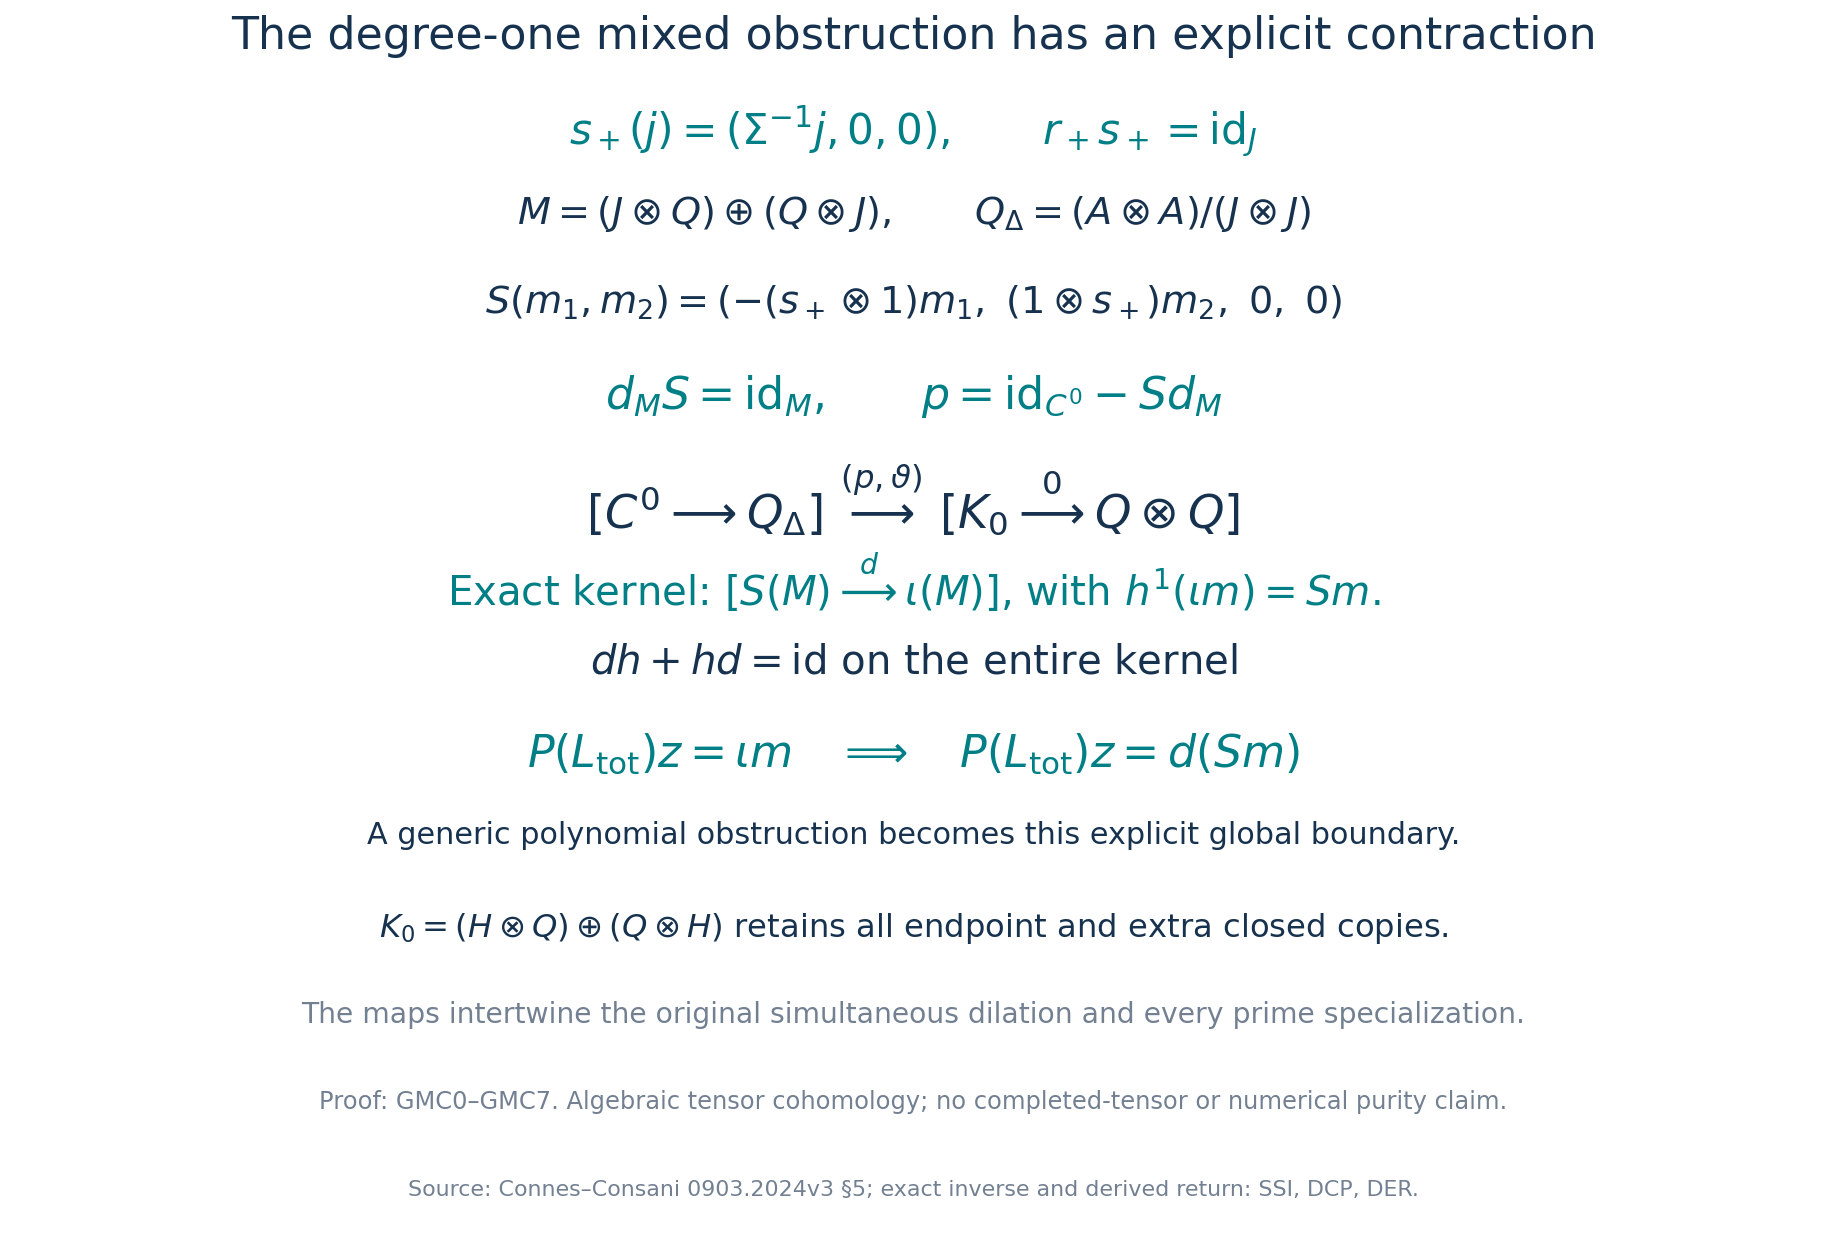
\includegraphics[keepaspectratio,alt={The global mixed contraction and exact boundary}]{GLOBAL_MIXED_RETURN_CONTRACTION.png}}
\caption{The global mixed contraction and exact boundary}
\end{figure}

Figure 5.
\href{https://github.com/KokunoYumeto/zeta-function-research-reader/blob/main/workbenches/splitzero-tandem/continuations/20260925-full-source-tensor-and-original-divisor/counterfactual/GLOBAL_MIXED_RETURN_CONTRACTION.md}{GMC0--GMC7}
constructs the displayed section from the already proved original
summation inverse, proves its equivariance, and supplies the full global
quasi-isomorphism and kernel homotopy. Every closed coefficient remains
in K\_0. The generic polynomial class is followed into the global
complex and becomes the displayed boundary. This is a proved mixed-term
vanishing calculation, not numerical purity of the remaining original Q.

Reproducible source: draw\_product\_sheaf\_pairing.py. All five final
PNGs were inspected. Eight exact finite-dimensional checks use the
coefficient fixture A=C\^{}4, J=C, W\_+=W\_-=C\^{}4; it is not
substituted for the original infinite-dimensional spaces. Five further
checks use the actual scalar matrices of the derived trace target,
making thirteen checks in total. No numerical test of RH is used.

Human sources: Alain Connes and Caterina Consani,
\href{https://arxiv.org/abs/0903.2024v3}{0903.2024v3 §5}; Ralf Meyer,
\href{https://arxiv.org/abs/math/0412277v3}{math/0412277v3}; Pierre
Deligne, \href{https://www.numdam.org/item/PMIHES_1980__52__137_0/}{Weil
II §§3.3.11, 3.4.8 and 3.6.1--3.6.3}. The author's TeX and the
separately identified Deligne transcription have exact reading/use
entries in the private ledger. The original source Z\_0, Z\_1/tau and
Z\_2 remain those supplied by the user. These figures concern
constructed receiving maps and make no numerical purity claim for
primitive tau.

\subsection{Publication source and dependency
links}\label{publication-source-and-dependency-links}

The source geometry is Alain Connes and Caterina Consani, \emph{Schemes
over F1 and zeta functions},
\href{https://arxiv.org/abs/0903.2024v3}{arXiv:0903.2024v3, §5}. The
weight-control comparison is Pierre Deligne, \emph{La conjecture de
Weil. II}, Publications mathematiques de l'IHES52 (1980),137-252,
\href{https://www.numdam.org/item/PMIHES_1980__52__137_0/}{§§3.3.11
and3.6}. Deligne material was read through the identified French
transcription and separately recorded peer source-page checks, not
Deligne-authored TeX. These sources are not asserted to contain the new
programme derivations. The
\href{https://github.com/KokunoYumeto/zeta-function-research-reader/blob/36a82ecca98addb8a98b48204e349737856c7223/workbenches/splitzero-tandem/continuations/20260924-cohomology-weight-and-character-lifts/BUILD_AND_REVIEW.md}{preceding
complete proof and reading record} records inherited source versions and
actual inspection limits. The investigator's corrected construction
remains attributed in the original text above.
